\subsection{Experimental Setup}
- describe i135
- describe benchmark set
- 900 seconds per instance
- describe IPC score
- refer to the detailed table of results at the end

\subsection{Improvements to CrowdHTN}
- putting numbers to memory savings and how many nodes we save from instantiation (also saves our loop detection!)
- percentage of search nodes saved by not representing search nodes beginning with an action
- percentage of world states saved by sharing them between nodes

\subsection{Search Algorithms}
In section \ref{improv: search algorithms} we presented four search algorithms that we implemented for CrowdHTN. Those algorithms are random DFS, heuristic DFS, A-star like and BFS. We have tested all four algorithms on our test instance set using 4 PEs and a local bloom filter without restarts for loop detection. The results of this test are visualized in figure \ref{figure: eval algorithm}, a summary of coverage and IPC score is presented in table \ref{table: eval algorithm}. \\
Overall, random DFS performed best, followed by heuristic DFS, A-star like search and finally BFS with our best algorithm, random DFS, solving almost twice as many instances and having twice the IPC score of our worst algorithm, BFS. Additionally, we observe a hit-or-miss behavior in both our DFS implementations where plans are either found almost immediately or not at all. Out of the 50 instances solved by random DFS, only 18 were solved in more than 1 and out of these 18 only 9 were solved in more than 10 seconds. BFS on the other hand solves 14 out of 30 instances in more than a second and 11 of these 14 in over 10 seconds. As such, while overall worse performing it does seem to scale better with runtime. \\
- heuristic is worse than random DFS
- due to the relatively simple nature of our heuristic, as our potential for precomputation is limited by malleability
- as expected, A-star performance lies between BFS and heuristic DFS

- discuss BFS reasons:
	- minimum plan depth due to lilotane
	- 
\begin{figure}
	\caption{Plotting the number of solved instances per runtime for CrowdHTN using DFS, heuristic DFS, A-star like search and BFS}
	\label{figure: eval algorithm}
	\centering
	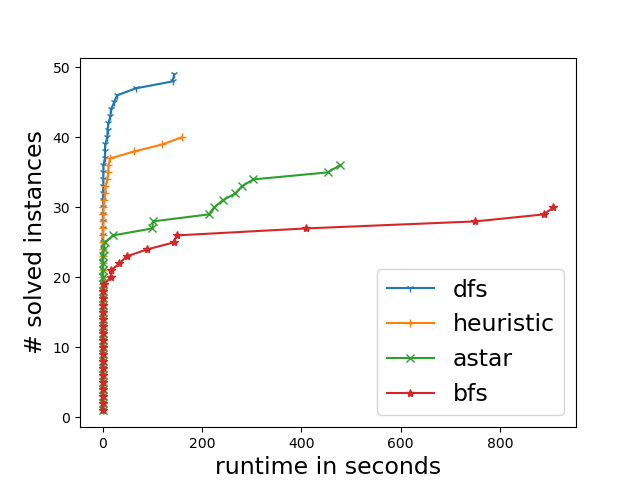
\includegraphics[width=0.5\textwidth]{images/final/search_algorithms.png}
\end{figure}
\begin{table}
	\caption{Coverage and IPC score of our search algorithms using 4 PEs and a local bloom filter}
	\label{table: eval algorithm}
	\centering
	\begin{tabular}{| l | r | r |}
		\hline
		Algorithm 		& Coverage & IPC Score \\
		\hline
		Random DFS 		& 41.7\%	& 43.09 \\ % 50
		Heuristic DFS 	& 33.3\%	& 35.60	\\ % 40
		A-star like 	& 38.3\%	& 27.13 \\ % 36
		BFS 			& 25.0\%	& 21.87	\\ % 30
		\hline
	\end{tabular}
\end{table}

\subsection{Scalability}
- show scaling on a nice instance

\subsection{Loop Detection}
- general loop detection:
- loop hit rate
- global loop hit rate
- performance of hash set vs bloom filter

\begin{figure}
	\caption{Plotting the number of solved instances per runtime for CrowdHTN comparing hash set and local bloom filter based loop detection on 32 and 64 PEs}
	\label{figure: eval loop detection}
	\centering
	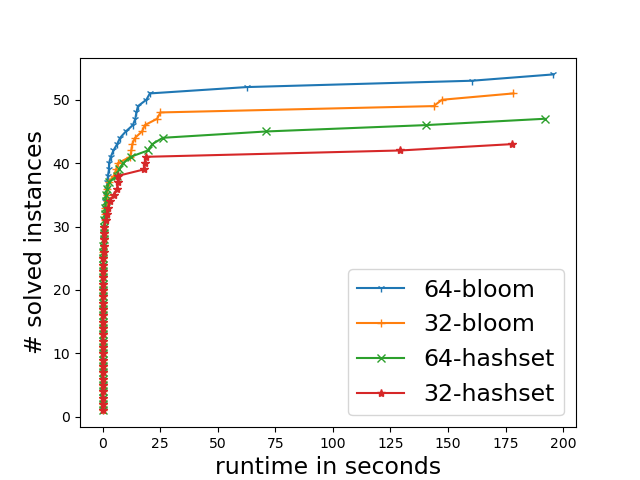
\includegraphics[width=0.5\textwidth]{images/final/loop_detection}
\end{figure}
\begin{table}
	\caption{Coverage and IPC score while using hash set and local bloom filter based loop detection on 32 and 64 PEs}
	\label{table: eval loop detection}
	\centering
	\begin{tabular}{| l | r | r |}
		\hline
		Configuration & Coverage & IPC Score \\
		\hline
		Hash set, 32 PEs	& 35.8\%	& 38.71 \\ % 43
		Hash set, 64 PEs	& 39.2\%	& 41.84 \\ % 47
		Bloom, 32 PEs		& 42.5\%	& 44.24 \\ % 51
		Bloom, 64 PEs		& 45.0\%	& 47.37 \\ % 54
		\hline
	\end{tabular}
\end{table}

\subsection{Probabilistic Restarts}
- test the probabilistic restarts
- with 900 seconds we expect $\sum_{t=1}^{899} \frac{1}{t} \approx 7.38$ restarts per run


\subsection{Global Loop Detection}
- test the global loop detection

\subsection{Malleable CrowdHTN}
- test the malleability

\subsection{Conclusion}
